% Describa el problema 
La Ingeniería de Requisitos (RE) constituye una fase crítica del ciclo de vida del desarrollo de software, cuyo objetivo es garantizar que las necesidades de todos los interesados 
sean capturadas, analizadas y documentadas con precisión antes de iniciar la construcción del sistema \cite{Wolf2026}.  Asegurar la calidad de estas especificaciones representa un 
desafío importante debido a su carácter no estructurado y a la dependencia de expertos humanos para su elaboración \cite{Wolf2026}.En la práctica actual, la creación del documento 
de Especificación de Requisitos de Software (SRS) sigue siendo una tarea predominantemente manual que consume tiempo excesivo, recayendo sobre los miembros más experimentados del 
equipo e impidiendo que destinen su esfuerzo a actividades de mayor valor \cite{Rahman2024}.

Esta situación se origina en la naturaleza ambigua del lenguaje natural empleado en las entrevistas, limitación reconocida explícitamente por el estándar IEEE 830-1998, 
que establece la necesidad de revisión independiente para identificar usos ambiguos antes de aceptar un SRS como válido \cite{doe2011recommended}, \cite{ieee1984ieee}. 
La ausencia de herramientas que guíen la estructuración formal del documento genera especificaciones incompletas, inconsistentes o no verificables \cite{ieee1984ieee}. 
dificultando especialmente la extracción de requisitos funcionales a partir de conversaciones informales, cuya omisión compromete atributos de calidad como rendimiento, 
seguridad y Conservabilidad \cite{Umar2024}, \cite{Mukaida2025}. A pesar del avance de los Modelos de Lenguaje de Gran Escala (LLMs), su uso individual presenta limitaciones 
en la gestión de contextos extensos y propensión a generar información incorrecta denominada "alucinaciones", agravando aún más el problema \cite{Rahman2024}.

Las consecuencias de una documentación deficiente son severas:los déficits detectados en fases tardías provocan retrabajos costosos que comprometen presupuesto 
y plazos \cite{Wolf2026}, 
debilitan la comunicación entre clientes y desarrolladores, e incrementan el riesgo de fracaso del proyecto \cite{Umar2024}. En este proceso intervienen variables 
críticas como la calidad semántica de los requisitos, completitud, consistencia y ausencia de ambigüedad\cite{Akhtar2025}, el tiempo invertido en la redacción del 
SRS y el grado de conformidad con el estándar IEEE 830-1998 \cite{ieee1984ieee}, \cite{Hoy2023}.

Desde el campo de la ingeniería, se propone el desarrollo de un sistema multi-agente basado en el Model Context Protocol e inteligencia artificial generativa, que 
especializa los LLMs en roles diferenciados de transcripción, análisis, clasificación y generación del documento SRS \cite{Guo2024},superando las limitaciones de los 
modelos individuales mediante inyección de contexto rico proveniente del audio de entrevistas y comunicación estructurada entre agentes y fuentes de datos externas \cite{Ray2025}. 
Este enfoque busca automatizar la transición entre el lenguaje natural hablado y la especificación técnica formal conforme al estándar IEEE 830-1998, reduciendo la carga operativa 
del equipo de ingeniería y elevando la calidad de la documentación producida.

\begin{figure}[H]
    \centering
    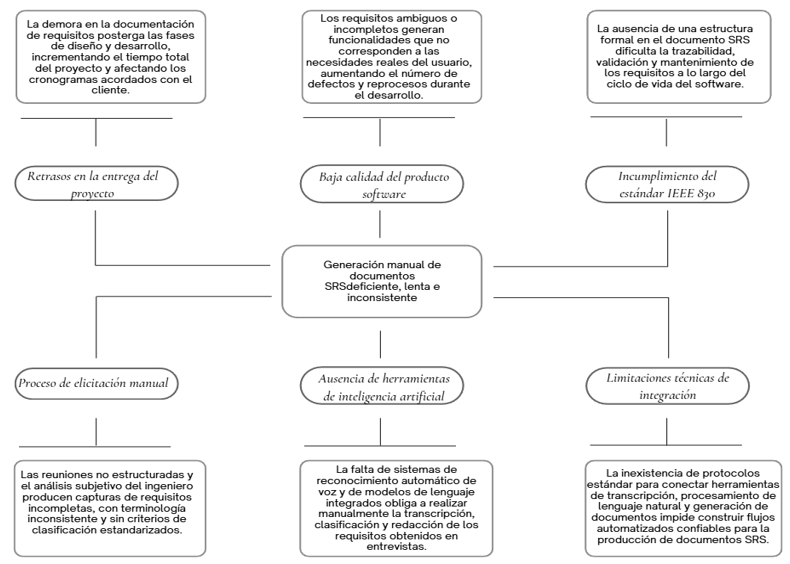
\includegraphics[width=0.8\linewidth]{ANTEPROYECTO/0.1-PROBLEMA/1.png}
    \caption[Análisis causal de la generación manual de documentos SRS] {Análisis causal de la generación manual de documentos SRS}
    \label{fig:Problema}
\end{figure}

